\documentclass[border=10pt]{standalone}

\usepackage{tikz}
\usepackage{tikzsymbols}
\usetikzlibrary{calc,patterns,shapes.geometric}

\def\centerarc[#1](#2)(#3:#4:#5){\draw[#1] ($(#2)+({#5*cos(#3)},{#5*sin(#3)})$) arc (#3:#4:#5);}

\begin{document}
	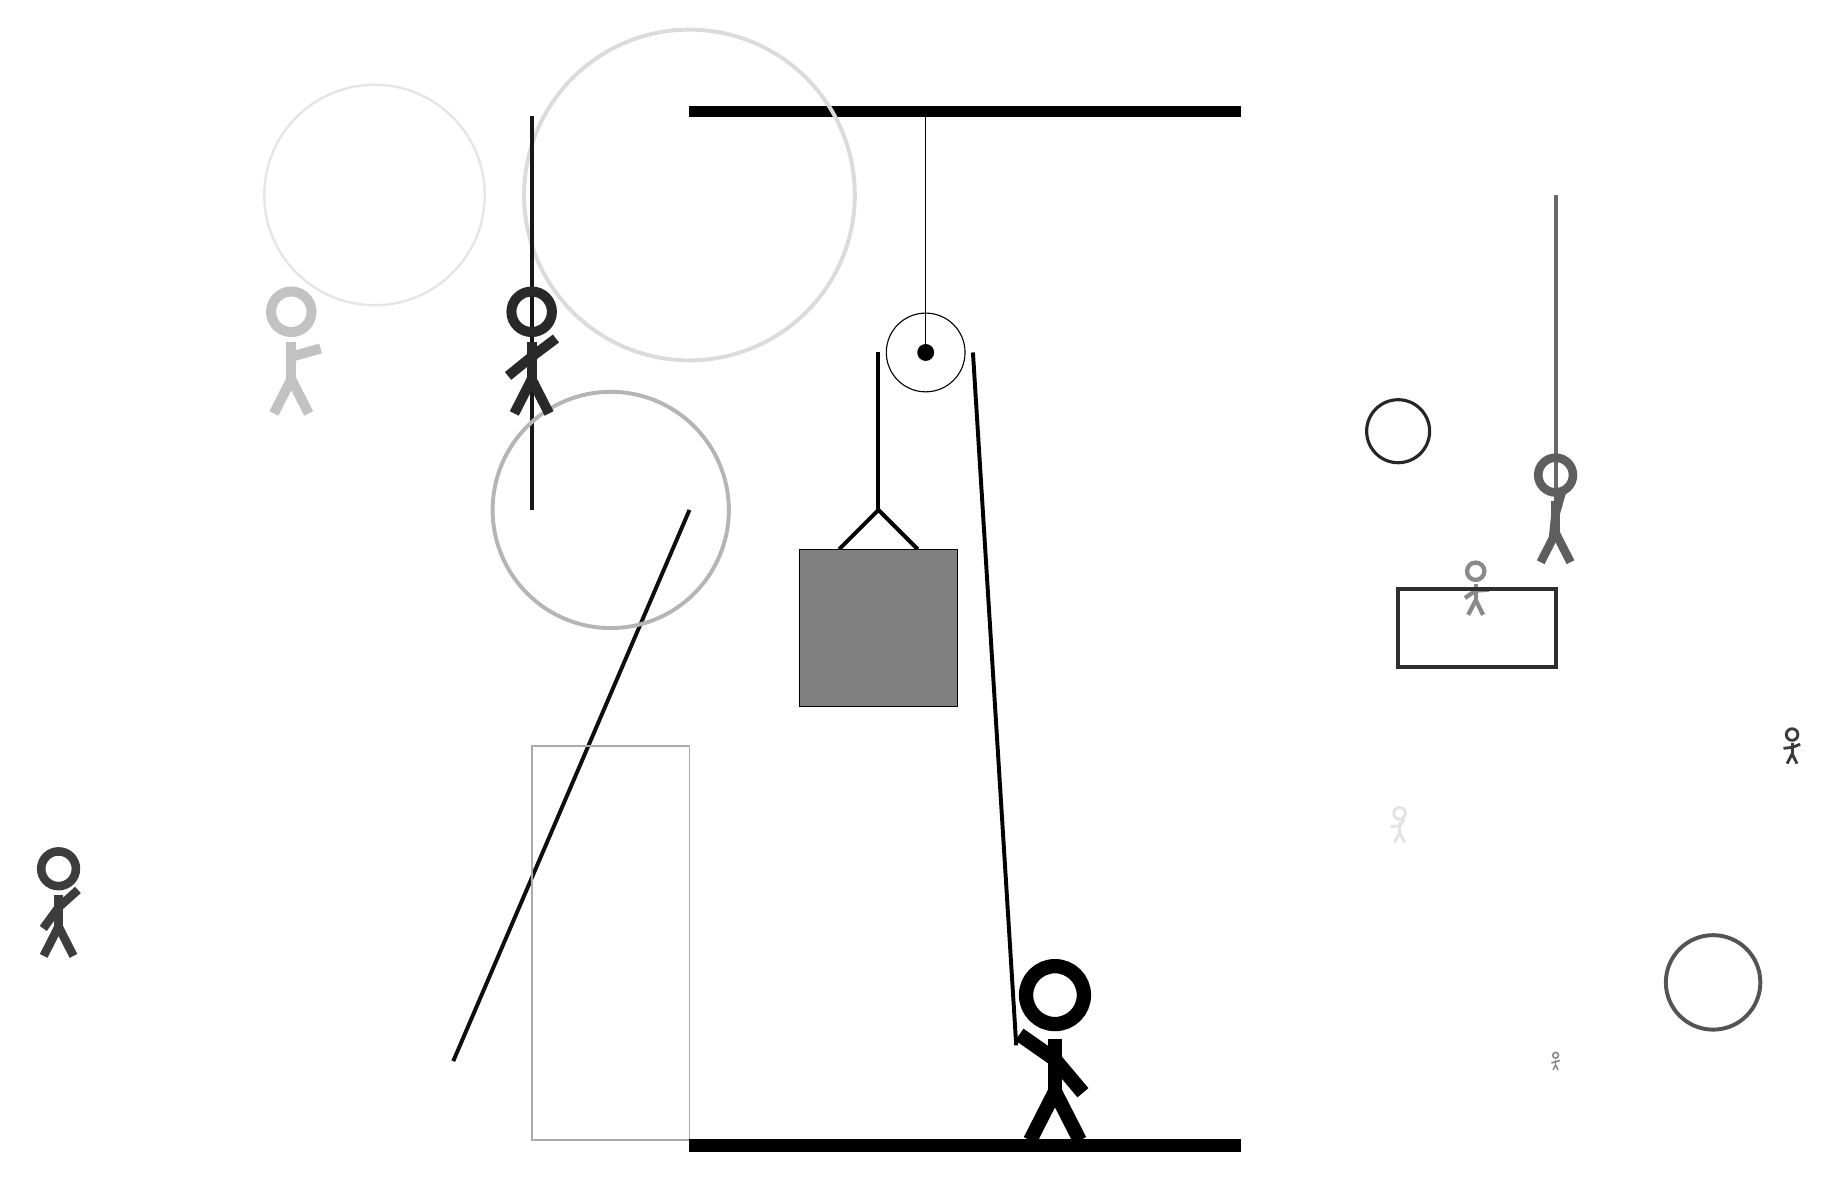
\begin{tikzpicture}
		%%%%% START %%%%%
		
		\draw[fill=black] (-2, 10) rectangle (5, 10.125);
		
		\draw (1, 7) circle (0.5);
		\draw[fill=black] (1, 7) circle (0.1);
		\draw (1, 10) -- (1, 7);
		
		\draw[line width=0.5mm] (-0.1, 4.5) -- (0.4, 5.0) -- (0.9, 4.5);
		\draw[fill=black!50] (-0.6, 4.5) rectangle (1.4, 2.5);
		
		\draw [line width=0.5mm, color=black!14](-2, 9) circle (2.1);
		
		\draw[line width=0.5mm, color=black!94](-2, 5) -- (-5, -2);
		\draw[line width=0.2mm, color=black!33] (-4, 2) rectangle (-2, -3);
		\node[line width=0.3mm, color=black!11] at (7, 1) {\Strichmaxerl[2][2][58]};
		
		\node[line width=0.4mm, color=black!76] at (-10, 0) {\Strichmaxerl[6][54][42]};
		
		\node[line width=0.3mm, color=black!77] at (12, 2) {\Strichmaxerl[2][6][21]};
		\draw[line width=0.5mm, color=black!59](9, 9) -- (9, 5);
		\node[line width=0.3mm, color=black!50] at (9, -2) {\Strichmaxerl[1][17][16]};
		\node[line width=0.7mm, color=black!24] at (-7, 7) {\Strichmaxerl[7][90][16]};
		\node[line width=0.3mm, color=black!46] at (8, 4) {\Strichmaxerl[3][35][4]};
		\node[line width=0.7mm, color=black!63] at (9, 5) {\Strichmaxerl[6][84][74]};
		\draw[line width=0.6mm, color=black!91] (-4, 10) rectangle (-4, 5);
		\draw [line width=0.5mm, color=black!67](11, -1) circle (0.6);
		
		\draw [line width=0.4mm, color=black!85](7, 6) circle (0.4);
		\draw [line width=0.5mm, color=black!29](-3, 5) circle (1.5);
		\draw [line width=0.3mm, color=black!10](-6, 9) circle (1.4);
		
		\draw[line width=0.5mm, color=black!82] (7, 4) rectangle (9, 3);
		
		\node[line width=0.6mm, color=black!84] at (-4, 7) {\Strichmaxerl[7][39][37]};
		
		\draw[line width=0.5mm] (0.4, 7) -- (0.4, 5.0);
		\centerarc[line width=0.5mm](1, 7)(0:180:0.6);
		\draw[line width=0.5mm](1.6, 7) -- (2.15, -1.8);
		
		\node at (2.6, -1.9) {\Strichmaxerl[10][-35][-50]};
		
		\draw[fill=black] (-2, -3) rectangle (5, -3.15);
		
		%%%%% END %%%%%
	\end{tikzpicture}
\end{document}